\documentclass[border=0pt]{standalone}

\usepackage{tikz}        % drawing macros
  \usetikzlibrary{math}
  \usetikzlibrary{calc}  % calculations
  \usetikzlibrary{arrows}  % arrowheads
  \usetikzlibrary{arrows.meta}  % arrowheads
  \usetikzlibrary{decorations.markings}
\usepackage{tikz-3dplot} % drawing macros 3d
\usepackage{pgfplots}
%\pgfplotsset{compat=1.18}

\begin{document}

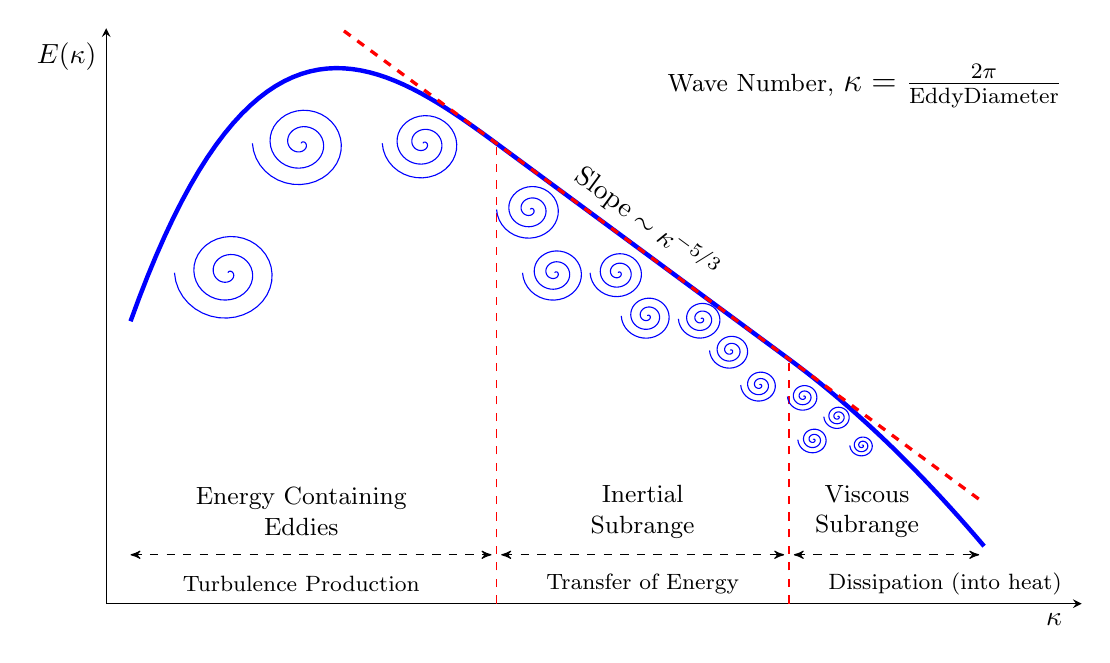
\begin{tikzpicture}[
declare function={
% Approximate the energy spectra using three cubic curve segments.
% Specify control points and slopes.
  x1 = 0.5 ; y1 = 6.0             ; s1 =  4.0;
  x2 = 4.0 ; y2 = 8.0             ; s2 = -5/4;
  x3 = 7.0 ; y3 = y2 + s2*(x3-x2) ; s3 =  s2;
  x4 = 9.0 ; y4 = 1.0             ; s4 = -2.0;
%
% Compute cubic curve fits for line segments.
  a0 = y1 ;
  a1 = s1 ;
  a2 = ( -2*a1 - s2 + 3*(y2-y1)/(x2-x1) ) / (x2-x1) ;
  a3 = (    a1 + s2 - 2*(y2-y1)/(x2-x1) ) / (x2-x1)^2 ;
  b0 = y2 ;
  b1 = s2 ;
  b2 = ( -2*b1 - s3 + 3*(y3-y2)/(x3-x2) ) / (x3-x2) ;
  b3 = (    b1 + s3 - 2*(y3-y2)/(x3-x2) ) / (x3-x2)^2 ;
  c0 = y3 ;
  c1 = s3 ;
  c2 = ( -2*c1 - s4 + 3*(y4-y3)/(x4-x3) ) / (x4-x3) ;
  c3 = (    c1 + s4 - 2*(y4-y3)/(x4-x3) ) / (x4-x3)^2 ;
%
% Define the composite curve as a function.
  engy(\x) =
      (\x<=x2)        * ( a0 + a1*(\x-x1) + a2*(\x-x1)^2 + a3*(\x-x1)^3 ) +
   and(\x>x2, \x<=x3) * ( b0 + b1*(\x-x2) + b2*(\x-x2)^2 + b3*(\x-x2)^3 ) +
      (\x>x3)         * ( c0 + c1*(\x-x3) + c2*(\x-x3)^2 + c3*(\x-x3)^3 ) ;
%
% Define the slope of the linear segment.
  slope(\x) = y2 + s2*(\x-x2);
%
% Define the eddy size as a function of wavenumber (x-axis position).
% Linear interpolation based on visually sizing the biggest/smallest eddies.
  eddyS(\x) = 1.00 + (0.20-1.00)*(\x-1.25)/(8.00-1.25);
%
% Define the swirling eddy.
% Define the eddy spiral radius, x, and y as a function of angle theta (deg).
%   Must scale by the plot aspect ratio for the eddies to appear circular.
  plotw     = 5.5;
  ploth     = 3.5;
  eddyR(\x) = 0.0 + 0.20 * \x / 360.;
  eddyX(\x) =      eddyR(\x)*cos(\x-90);
  eddyY(\x) = -1.0*eddyR(\x)*sin(\x-90) * plotw/ploth;
}
]% end tikzpicture optional args
%
% Create the plot axes.
\begin{axis}
[
  width=5.5in, height=3.5in, clip=false,
  axis x line=middle,
  axis y line=middle,
  samples=101, domain=0.25:9.0,
%
% Linear plot axes. Each 0:10 to ease manual placement.
  xmin=0, xmax=10, xtick={1,...,9}, xmajorticks=false, xticklabels={},
  ymin=0, ymax=10, ytick={2,4,6,8}, ymajorticks=false, yticklabels={},
%
%
% Cannot get axis labels (titles) to place properly when ticks are off.
%
% x label style={at={(axis description cs:0.95,-0.50)},anchor=north},
% x label style={at=(0.95,-0.50),anchor=north},
% xlabel=$\log{\kappa}$, % xlabel near ticks,
%
% y label style={at={(axis description cs:-0.01,0.95)},anchor=east},
% ylabel=$\log{E(\kappa)}$, % ylabel near ticks,
%
]% end axis optional args
%
%
% Fake axis titles. Difficulty placing actual titles on outside end axis.
  \node[anchor=      east] at (axis cs:-0.00, 9.50) {${E(\kappa)}$};
  \node[anchor=north east] at (axis cs: 9.90,-0.00) {${\kappa}$} ;
%
% Added nomenclature.
  \node[anchor=east] at (axis cs: 9.90, 9.00) {{\small Wave Number,} {\large ${\kappa}=\frac{2\pi}{\mathrm{Eddy Diameter}}$}} ;
%
% Plot the energy function.
  \addplot[blue,ultra thick]{engy(x)};
%
% Plot the slope of the energy function.
  \addplot[red,dashed,very thick,domain=0.25:9.0,restrict y to domain = 0:10]%
    {slope(x)}
    node[pos=0.45,sloped,anchor=south,black]{$\mathrm{Slope}\sim\kappa^{-5/3}$};
%
% Vertical dashed lines for different regions.
% \pgfplotsinvokeforeach{x2,x3}
% {
%   \addplot[red,dashed] coordinates {(#1,0) (#1,10)};
% } 
  \addplot[red,dashed] coordinates {(x2,0) (x2,y2)};
  \addplot[red,dashed] coordinates {(x3,0) (x3,y3)};
%
% Horizontal arrows for different regions.
\begin{scope}[black,dashed,>={stealth'[scale=10]}]
  \addplot[<->] coordinates {(   0.25,0.85) (x2-0.05,0.85)};
  \addplot[<->] coordinates {(x2+0.05,0.85) (x3-0.05,0.85)};
  \addplot[<->] coordinates {(x3+0.05,0.85) (x4-0.05,0.85)};
\end{scope}
%
% Lables for different regions.
\begin{scope}[font=\small]
  \node[align=center] at (axis cs:2.00,1.60) {Energy Containing\\Eddies};
  \node[align=center] at (axis cs:5.50,1.60) {Inertial\\Subrange};
  \node[align=center] at (axis cs:7.80,1.60) {Viscous\\Subrange};
\end{scope}
%
% Description for different regions.
\begin{scope}[font=\footnotesize]
  \node[align=center] at (axis cs:2.00,0.35) {Turbulence Production};
  \node[align=center] at (axis cs:5.50,0.35) {Transfer of Energy};
  \node[align=center] at (axis cs:8.60,0.35) {Dissipation (into heat)};
\end{scope}
%
% Plot eddies. Manually placed.
\begin{scope}[blue]
  \addplot[domain=0:360*2.75]({1.25+eddyS(1.25)*eddyX(x)},
                              {5.75+eddyS(1.25)*eddyY(x)}) ;
  \addplot[domain=0:360*2.75]({2.00+eddyS(2.00)*eddyX(x)},
                              {8.00+eddyS(2.00)*eddyY(x)}) ;
  \addplot[domain=0:360*2.75]({3.25+eddyS(3.25)*eddyX(x)},
                              {8.00+eddyS(3.25)*eddyY(x)}) ;
  %
  \addplot[domain=0:360*2.75]({4.35+eddyS(4.35)*eddyX(x)},
                              {6.85+eddyS(4.35)*eddyY(x)}) ;
  \addplot[domain=0:360*2.75]({4.60+eddyS(4.60)*eddyX(x)},
                              {5.75+eddyS(4.60)*eddyY(x)}) ;
  \addplot[domain=0:360*2.75]({5.25+eddyS(5.25)*eddyX(x)},
                              {5.75+eddyS(5.25)*eddyY(x)}) ;
  \addplot[domain=0:360*2.75]({5.55+eddyS(5.55)*eddyX(x)},
                              {5.00+eddyS(5.55)*eddyY(x)}) ;
  \addplot[domain=0:360*2.75]({6.10+eddyS(6.10)*eddyX(x)},
                              {4.95+eddyS(6.10)*eddyY(x)}) ;
  \addplot[domain=0:360*2.75]({6.40+eddyS(6.40)*eddyX(x)},
                              {4.40+eddyS(6.40)*eddyY(x)}) ;
  \addplot[domain=0:360*2.75]({6.70+eddyS(6.70)*eddyX(x)},
                              {3.80+eddyS(6.70)*eddyY(x)}) ;
  %
  \addplot[domain=0:360*2.75]({7.15+eddyS(7.15)*eddyX(x)},
                              {3.60+eddyS(7.15)*eddyY(x)}) ;
  \addplot[domain=0:360*2.75]({7.25+eddyS(7.25)*eddyX(x)},
                              {2.85+eddyS(7.25)*eddyY(x)}) ;
  \addplot[domain=0:360*2.75]({7.50+eddyS(7.50)*eddyX(x)},
                              {3.25+eddyS(7.50)*eddyY(x)}) ;
  \addplot[domain=0:360*2.75]({7.75+eddyS(7.75)*eddyX(x)},
                              {2.75+eddyS(7.75)*eddyY(x)}) ;
\end{scope}
\end{axis}
\end{tikzpicture}

\end{document}
